\documentclass[12pt]{article}

\usepackage{sbc-template}

\usepackage{graphicx,url}

\usepackage[brazil]{babel}   
%\usepackage[latin1]{inputenc}  
\usepackage[utf8]{inputenc}  
% UTF-8 encoding is recommended by ShareLaTex
\usepackage{multirow}

\sloppy

%\title{Instructions for Authors of SBC Conferences\\ Papers and Abstracts}
\title{Desenvolvimento de um Middleware para Comunicação via Web Services e sua Aplicação  em uma API de Processamento Digital de Imagens}
\author{Fernando Henrique Alves\inst{1}}

\address{
  Centro de Ciências Exatas e Naturais\\
  Universidade Federal Rural do Semi-Árido (UFERSA) -- Mossoró, RN -- Brazil
  \email{fernandofha01@gmail.com}
}

\begin{document} 

\maketitle

\begin{abstract}
  The technological evolution has been making the Distance
  Education accessible for a greater number of citizens anytime and anywhere.
  The potential increase of the supply for mobile devices integrated to mobile
  learning environments allows that the information comes out of the physical
  environment, creating opportunities for students and teachers to create
  geographically distributed learning scenarios. However, many applications
  developed for these environments remain isolated from each other and do not
  become integrated sufficiently into the virtual learning environments (AVA).
  This paper presents an interoperability model between mobile devices and
  distinct AVA based on webservices.
\end{abstract}

\begin{resumo} 
  A evolução tecnológica tem tornado a Educação a Distância
  acessível para um maior número de cidadãos em qualquer hora e em qualquer
  lugar. O aumento potencial da oferta de dispositivos móveis integrados a
  ambientes de aprendizado móvel permite que a informação saia dos ambientes
  físicos das instituições de ensino, oportunizando a alunos e professores
  criarem cenários de aprendizagem geograficamente distribuídos. Entretanto,
  muitos dos aplicativos desenvolvidos para estes ambientes ainda permanecem
  isolados uns dos outros e não se integram de maneira suficiente aos ambientes
  virtuais de aprendizagem (AVA). Este artigo apresenta um modelo de
  interoperabilidade entre dispositivos móveis e AVA distintos baseado em
  webservices.
\end{resumo}


\section{Introdução/Motivação}

Com a evolução da tecnologia, foram desenvolvidas várias facilidades para o ser humano. 
Dentre elas, a Computação e a Internet se destacam por automatizar tarefas, reduzir
custos, distância e tempo para realizar a troca de vários tipos de informação. 

Toda área, seja ela educação, comércio, medicina ou militar, exige troca de informação para seu funcionamento. 
Um dos mais populares modos de comunicação de dados via internet é através do uso de um web service. 
Web services podem ser definidos como aplicações cliente/servidor que se utilizam da comunicação 
através da internet, por meio do protocolo HTTP (HyperText Transfer Protocol), para prover serviços 
entre softwares que estejam executando em diferentes plataformas. Essas aplicações fazem uso do padrão 
XML (eXtensible Markup Language) para prover descritores que são interpretados automaticamente 
por outros sistemas, permitindo assim que diversos programas simples possam interagir uns com os 
outros para, em conjunto, fornecer soluções mais complexas e sofisticadas(DEVMEDIA).

Nos últimos anos, têm-se acompanhado a disponibilização de um grande número de sistemas 
computacionais com um considerável conjunto de recursos que satisfaçam as necessidades de 
desenvolvedores de software. Esse aumento do poder computacional gera um desejo de tratar 
problemas de maior escopo por parte de programadores e pesquisadores, e uma das áreas que podem 
se beneficiar de tal avanço é a de Processamento Digital de Imagens (PDI), pois a popularização 
de dispositivos de aquisição e armazenamento de mídias digitais, como imagens e vídeos, faz 
crescer a demanda por software capaz de manipulá-las. Neste contexto, bibliotecas de software 
podem incorporar implementações de métodos que são a base comum para a manipulação de imagens e 
vídeos a fim de minimizar erros de codificação, diminuir o custo e o tempo de produção. 
Com a disseminação da internet e da consequente e inevitável necessidade de troca de informação, 
as aplicações e sistemas desenvolvidos hoje em dia precisam 
atender a certas condições do cenário atual, essas condições dizem respeito às características 
de execução dos softwares de forma distribuída, rápida e portável. 

Diante da necessidade de permitir que uma biblioteca de PDI atenda a tais requisitos, surge a
possibilidade de implementar uma ferramenta, independente de plataforma, para a
disponibilização de suas funcionalidades.

Para chegar à ferramenta, a solução está implementada em Linguagem
Java, com auxílio de uma ferramenta denominada JERSEY, baseada na arquitetura
SOA, mais especificamente em Serviço Web seguindo o conceito REST, do inglês
Representational State Transfer (Transferência do Estado Representacional), o qual
foi proposto por Roy T. Fielding em sua dissertação de doutorado, publicada no ano
2000. (SANDOVAL, 2009)

Este tipo de Serviço Web utiliza-se do protocolo HTTP para realizar a troca
de mensagens entre clientes e servidor. Outra característica importante é a forma de
redirecionamento de serviços, realizado através de um endereçamento URI
específico. (RICHARDSON; RUBY, 2007)

Aliando todos os fatores e tecnologias apresentados anteriormente, torna-se
possível o desenvolvimento de uma arquitetura baseada em Serviços Web,
fornecendo uma plataforma que disponibiliza serviços de uma API de processamento digital de imagens
com baixos custos computacionais, ou seja, baixo consumo de memória e processamento.

\section{Referencial Teórico} \label{sec:firstpage}

\subsection{Middleware}

Para Coulouris (2005) o middleware “é um termo aplicado a uma camada de software
que fornece uma abstração da programação, assim como o mascaramento de
heterogeneidade das redes, do hardware, de sistemas operacionais e linguagens de
programação subjacentes”. Tal camada configura funções de identificação, autorização,
autenticação, segurança, entre outras. O middleware implementa a comunicação e o
compartilhamento de recursos e aplicativos distribuídos.
Um middleware forma uma camada entre aplicações e plataformas distribuídas
cuja finalidade é proporcionar um grau de transparência de distribuição. [Tanenbaum,
2007]
Neste trabalho pretende-se fazer middleware de modo que sejam simples as
configurações, adaptações e personalizações da aplicação conforme sejam necessárias.

\subsection{Webservice}

Com o surgimento da comunicação através das redes de computadores e da necessidade
de diferentes softwares se comunicarem entre si surgiu o conceito de Webservice (WS).
Os Webservices permitem que sistemas desenvolvidos em diferentes linguagens,
sendo executados em diversas plataformas, transmitam e recebam informações
padronizadas entre si, permitindo uma interação entre os dispositivos, mais abrangente
que qualquer outra tecnologia de computação distribuída existente.
Segundo Kalin (2009) Webservice é um tipo de aplicação para web distribuída,
cujos componentes podem ser aplicados e executados em dispositivos distintos.
Configura-se como um mecanismo de comunicação que permite a interoperabilidade
entre sistemas. Para Kreger (2001) um Webservice descreve uma coleção de operações
que são acessíveis pela rede através de mensagens XML (eXtensible Markup Language)
padronizadas. Porém existe a tecnologia JSON (Javascript Object Notation) que
também possibilita a troca de mensagens de forma mais leve. O uso de Webservice
possibilita que aplicações desenvolvidas em plataformas e linguagens diversificadas
troquem informações padronizadas permitindo a interação entre elas com rapidez,
facilidade e baixo custo, conforme ilustrado na Figura 1.

\begin{figure}[ht]
	\centering
	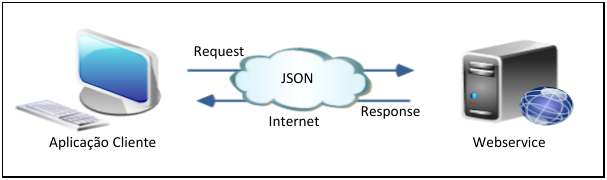
\includegraphics[width=.8\textwidth]{figura1.png}
	\caption{Troca de informações entre uma aplicação cliente e um WebService}
	\label{fig:exampleFigura1}
\end{figure}

Souza (2004) explica que os Webservices utilizam tecnologias que permitem que
os serviços sejam disponibilizados pela WEB transportando e transformando dados
entre aplicações com base em XML ou JSON. Nesse contexto, o XML e JSON além de
funcionarem como padrão para troca de mensagens também têm o papel de definir os
serviços. Sua sintaxe especifica como os dados são representados, transmitidos e
detalhes de como são publicados e descobertos.

Existem basicamente, dois grupos de serviços web: os serviços baseados em SOAP (Simple Object Access Protocol) e os REST (Representational
State Transfer ). Um serviço baseado em SOAP entregue sobre HTTP é um caso especial dos serviços REST. O foco deste trabalho está na criação e utilização de um web service do grupo REST, devido a sua popularização, e ferramentas auxiliares disponíveis para uso.

\subsubsection{REST - Representational State Transfer}

Descrito por Fielding (2000), REST é um modelo de arquitetura de software distribuído, baseado em comunicação via rede.
%Um sistema no estilo REST é denominado RESTful e possui as seguintes características:
Para a implementação de um sistema RESTful não há a necessidade da criação de novos protocolos ou tecnologias, pois o mesmo é suportado em qualquer arquitetura de rede.
Enquanto o SOAP é um protocolo de mensagens, o REST é um estilo de arquitetura
de software para sistemas hipermídia distribuídos, conhecidos como recursos. Um recurso RESTful é qualquer coisa que possua um endereço através da web, ou seja, sistemas em que as hipermídias são armazenadas em uma rede e interconectadas através de hiperlinks podendo ser acessados e transferidos entre clientes e servidores.
O núcleo da abordagem REST consiste na utilização dos métodos HTTP, que correspondem às operações CRUD (Create, Read, Update, Delete). Cada requisição HTTP inclui um dos métodos apresentados na tabela 2.1 para indicar qual a operação CRUD que deve ser realizada sobre o recurso.
\begin{table}[ht]
	\centering
	\caption{Métodos HTTP e operações CRUD}
	\label{tab:Table1}
	\smallskip
	\begin{tabular}{ |l|l| }
		\hline
		POST & Cria um novo recurso a partir dos dados requisitados \\ \hline
		GET & Lê um recurso \\ \hline
		PUT & Atualiza um recurso a partir dos dados requisitados \\ \hline
		DELETE & Remove um recurso \\
		\hline
	\end{tabular}
\end{table}

Em termos gerais, um cliente RESTful emite um pedido que envolve um recurso, como
por exemplo, um pedido de alteração. Se este pedido for bem sucedido, uma representação
do recurso é transferido do servidor que hospeda o recurso para o cliente que emitiu o
pedido [Kalin 2009].


\subsection{Processamento Digital de Imagens(PDI)}

Uma imagem pode ser definida por uma função bidimensional f (x,y) em que x e y são um par de coordenadas espaciais e o valor de f representa a intensidade da
imagem naquele ponto. Quando x, y e os valores das intensidades de f são todos finitos e em quantidades discretas, pode-se dizer que a imagem é uma imagem
digital. Os elementos constituintes das imagens são denominados pixels. O PDI refere-se à utilização de métodos que manipulam imagens digitais e que geram
como resultado outras imagens digitais. Esta manipulação envolve a utilização dos pixels da imagem de entrada para a geração de novos pixels que formam a
nova imagem de obtida [4].

Na maioria dos casos, os métodos que se deseja implementar para a manipulação das imagens são mapeamentos, considerando a utilização de uma matemática
básica ou avançada, que utilizam as posições e os valores dos próprios pixels. Entretanto, quando os programadores se deparam com o desenvolvimento de
programas que processam imagens, eles devem se preocupar com outras tarefas que não são estão ligadas à essência do PDI. Exemplos destas tarefas são dados
pela escolha e utilização de bibliotecas para a leitura e gravação de arquivos, criação de interface gráfica ou aplicação de testes para verificação do que foi
implementado. Estas nuâncias de implementação podem ser abstraídas através do uso de uma biblioteca específica que faça a abstração destas tarefas [4, 5].

\subsection{Application Programming Interface(API)}

\subsection{API em Desenvolvimento}


\section{Mecanismo de chamada de serviço remoto (RSI)}

Esta sessão está destinada a descrever a arquitetura e funcionamento do Middleware proposto, bem como as tecnologias envolvidas em sua implementação.

%A função de um middleware é tornar possível a comunicação entre aplicações que
%não se comunicam diretamente. Para o contexto deste trabalho, que é o de promover a disponibilização das funcionalidades de uma API de PDI, o uso de um middleware é de fundamental
%importância, pois torna possível para que programadores, o torna flexível para novas possibilidades de comunicação com outras
%funcionalidades dos AVA, além da possibilidade de registrar o log de transações
%realizadas entre as partes e outras questões relacionadas à segurança. O middleware foi 
%desenvolvido baseado num padrão de interoperabilidade que permite a comunicação
%com diversos AVA. 

A figura 2 representa o diagrama da estratégia de comunicação que
foi desenvolvida em duas etapas: entre a aplicação cliente e o Middleware via Web Services e entre
o Middleware e a API de PDI desenvolvida via linha de comando, esta, que por sua vez, está localizada no mesmo servidor do web service.

Para a troca de informações adotou-se o JSON (JavaScript Object Notation). O
JSON é um formato de interconexão de dados utilizado em ambientes cliente-servidor
que possibilita o desenvolvimento nas mais variadas linguagens. O JSON atualmente
vem sendo utilizado como linguagem padrão para comunicação entre sistemas nas mais
diversas plataformas. A disponibilidade de bibliotecas e o desempenho proporcionado
pela simplicidade da transmissão de dados utilizando JSON influenciaram na decisão
por utilizá-lo.

A interoperabilidade entre a aplicação cliente e a biblioteca de PDI, conforme ilustrado na Figura 2, é
realizado da seguinte forma:
\begin{itemize}
	\item A aplicação cliente se conecta ao web service através da URL de acesso a algum serviço disponibilizado pelo mesmo, informando junto com a requisição, a imagem alvo a qual se deseja realizar tal transformação, codificada no formato base64;
	\item O middleware recebe a requisição, decodifica a imagem requisitada, salva-a no disco, e realiza uma chamada via linha de comando para o sistema operacional do servidor, passando como parâmetro o caminho da imagem salva, e o tipo de transformação que se deseja realizar na mesma, para que a API possa realizar seu trabalho;
	\item Após realizar seu processamento, a API retorna para o middleware como resultado de execução, a imagem transformada e codificada no formato base64;
	\item O middleware por fim, retorna para a aplicação cliente do serviço, um código de status da requisição, representando o sucesso ou insucesso da operação, em conjunto com uma mensagem informando se houve qualquer erro em algum dos passos anteriores, e caso todo o processo tenha sido realizado com sucesso, retorna também a imagem processada pela API, também no formato base64.
\end{itemize}

\begin{figure}[ht]
	\centering
	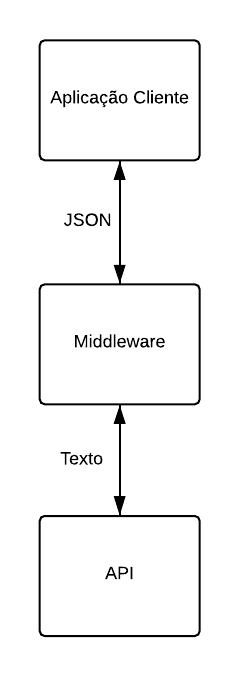
\includegraphics[width=.2\textwidth]{modelo-comunicacao.png}
	\caption{Modelo de Comunicação}
	\label{fig:Figura2}
\end{figure}

Para que o processo funcione adequadamente, a API precisa estar ao alcance do web service, ou seja, localizada no mesmo servidor, e também é necessário que a mesma implemente a forma padronizada de comunicação descrita anteriormente: enviar como resposta à suas chamadas de funções, uma imagem codificada no formato base64, para que o
middleware consiga se conectar à mesma e, dessa forma, interagir com as aplicações clientes conforme o esperado.

O middleware será executado em um servidor de aplicação. Este servidor
é responsável por estabelecer a comunicação com as aplicações clientes que desejem utilizar os serviços da API. 
A desvantagem é que recursos computacionais de um servidor serão alocados para o middleware, porém, como vantagens teremos a flexibilidade, melhoria no desempenho, manutenibilidade e disponibilidade do serviço.

A utilização das funcionalidades da API de forma direta, necessitando de tê-la instalada na própria máquina do utilizador, traria alguns inconvenientes, sendo eles:
\begin{itemize}
	\item O usuário necessitar instalar novas versões da mesma à medida que novas funcionalidades forem sendo adicionadas;
	\item Dependência de plataforma, uma vez que para se comunicar corretamente com a biblioteca de programação, o usuário necessita utilizar a mesma linguagem de programação com a qual a mesma fora implementada;
	\item Restrição de utilização da biblioteca à medida que os recursos da máquina do usuário foram ficando mais escassos, uma vez que todo o processamento da API será feito no computador do usuário.
\end{itemize}
%O uso do MiddleWare desonera o consumo da bateria e o processamento do aparelho que esteja executando o mesmo, ampliando sua performance.

O middleware possui a implementação e uso de três serviços através dos quais será possível realizar diversas operações de troca de informações.
Todos os serviços têm somente um parâmetro de entrada (request) e um parâmetro de saída (response) de tipos que encapsulam as informações necessárias para realizar as requisições e o resultado da operação. Os serviços são descritos a seguir:

\textit{ListFilters}: Operação destinada a realizar consultas dos filtros disponíveis para aplicação;

\textit{GreenFilter}: Operação destinada a realizar a aplicação do filtro de cor verde na imagem requisitada;

\textit{BlackAndWhiteFilter}: Operação destinada a realizar a aplicação do filtro de cores preto e branco na imagem requisitada.

A definição dos elementos de comunicação – ou objetos de comunicação – é
determinante para o sucesso de todo o processo de comunicação, que inicia na requisição da aplicação cliente, passa pelo middleware, chega na API, e finaliza na resposta final do web service. Esses objetos são as estruturas de dados que carregam as informações necessárias para consumir e responder um WS.
A dinâmica de comunicação é realizada da seguinte forma: a aplicação cliente realiza uma requisição encapsulando um objeto de comunicação que é processado pelo web service. Em seguida, o WS realiza uma chamada à função requisitada pelo cliente à API, esta que por sua vez, realiza seu processamento, e envia uma resposta ao WS, que, por fim, responde à requisição do cliente através de um outro objeto de comunicação.

Por exemplo: para consumir o serviço GreenFilter a aplicação cliente requisita através do objeto de comunicação Request os dados da imagem codificada. Em seguida, o serviço GreenFilter envia a resposta com o objeto de comunicação Response.

A tabela 1 representa um exemplo da estrutura de dados de um objeto de
comunicação exemplificado no formato JSON.

\begin{table}[ht]
	\centering
	\caption{Descrição dos atributos de comunicação}
	\label{tab:Table2}
	\smallskip
	\begin{tabular}{ |l|l|l| }
		\hline
		Objeto de Comunicação & Atributos & Exemplo (JSON) \\ \hline
		Request & Img: texto & \{“img" : “/9j/4AAQSkZJRgABAQAAAQAB"\} \\ \hline
		\multirow{3}{*}{Response} & Status: inteiro & \{“Status": 1, \\
		& Msg: texto & “Msg":“Sucesso", \\
		& Img: texto & “Img":“/9j/4AAQSkZJRgABAQAAAQAB"\} \\
		\hline
	\end{tabular}
\end{table}

A figura 3 representa o diagrama de sequência para o consumo do serviço GreenFilter:
\begin{figure}[ht]
	\centering
	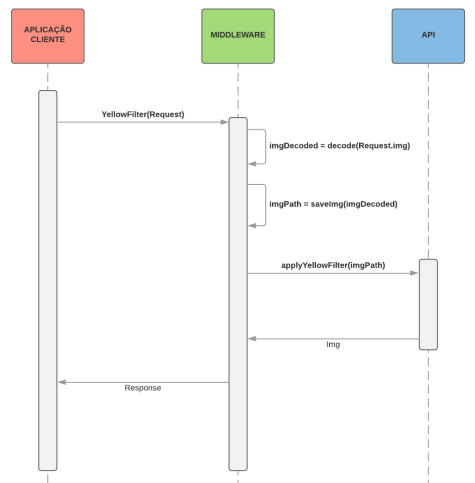
\includegraphics[width=.7\textwidth]{ds-yellow-filter.png}
	\caption{Diagrama de Sequência - YellowFilterService}
	\label{fig:Figura3}
\end{figure}


falar sobre as tecnologias envolvidas em sua implementação: Java EE, Jersey, Maven, JSON, base64, http...

\section{Estudo de caso}

Nesta sessão, serão descritos os passos necessários para a realização de consumo dos serviços da API por meio da comunicação com o Middleware, mostrando o desenvolvimento de uma aplicação cliente como estudo de caso.

A escolha da linguagem JavaScript como base para o desenvolvimento da aplicação cliente, se deu mais pela necessidade de demonstrar a independência de plataforma que o Middleware nos proporciona, e também pelo fato de que atualmente JavaScript é uma das linguagens mais conhecidas e utilizadas ao redor do mundo.

\section{Considerações Finais}


Bibliographic references must be unambiguous and uniform.  We recommend giving
the author names references in brackets, e.g. \cite{knuth:84},
\cite{boulic:91}, and \cite{smith:99}.

The references must be listed using 12 point font size, with 6 points of space
before each reference. The first line of each reference should not be
indented, while the subsequent should be indented by 0.5 cm.

SANDOVAL, Jose. RESTful Java Web Services. Birmingham: Packt Publishing,
2009.

RICHARDSON Leonard; RUBY, Sam. RESTful Web Services. Sebastopol: O'Reilly,
2007.

https://www.devmedia.com.br/introducao-a-web-services-restful/37387

\bibliographystyle{sbc}
\bibliography{sbc-template}

\end{document}
